\ylDisplay{Läätse skeem} % Ülesande nimi
{Tundmatu autor} % Autor
{piirkonnavoor} % Voor
{2014} % Aasta
{P 10} % Ülesande nr.
{3} % Raskustase
{
% Teema: Valgusõpetus
\ifStatement
Joonisel on kujutatud kaks sellist kiirt, mis lähtuvad punktvalgusallikast $A$ ning on läbinud läätse. Lääts asub sirgel $S$. Konstrueerige läätse fookuse asukoht.
\begin{center}
	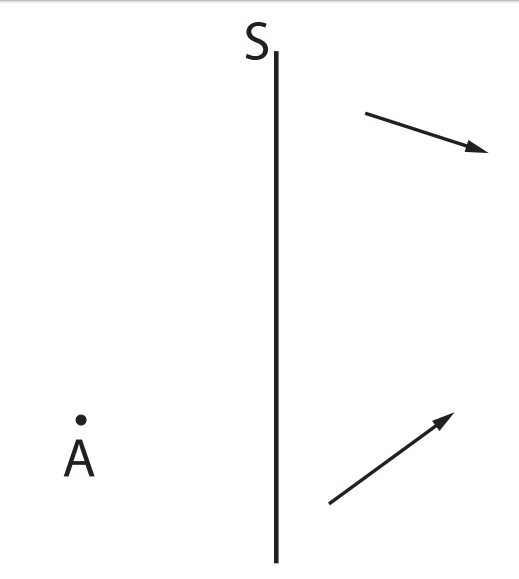
\includegraphics[width=0.5\linewidth]{2014-v2p-10-yl.PNG}
\end{center}
\fi
\ifHint
Lahenduseks piisab korrektse joonise olemasolust. Läbi läätse liikuvate kiirte lõikepunkti abil on võimalik konstrueerida fookust läbiva kiire liikumine.
\fi
\ifSolution
Olemasolevate kiirte pikendused lõikuvad punktis $A'$ , mis on punktvalgusallika $A$ kujutiseks. Läätse keskpunkti $O$ saame kätte, kui tõmbame sirge läbi punktide $A$ ja $A'$. Optiline peatelg on risti läätse tasandiga $S$ ning läbib punkti $O$. Läätse fookuse $F$ leiame, kui joonistame valgusallikast $A$ kiire AB, mis on parallelne optilise peateljega ning peale läätse läbimist peab ta läbima punkti $A'$.
\begin{center}
	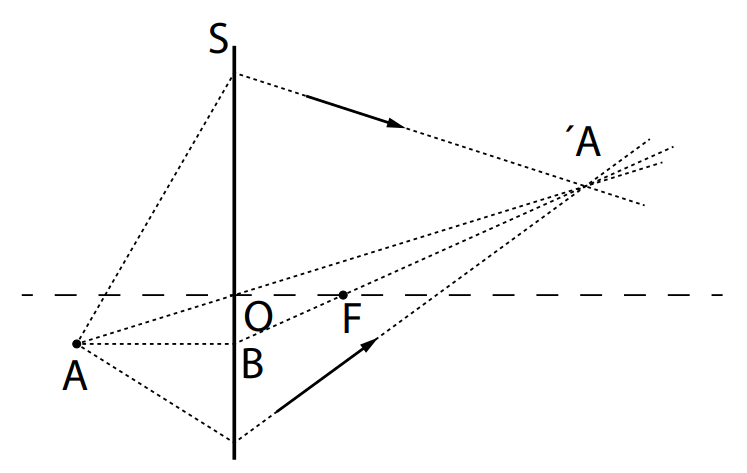
\includegraphics[width=0.5\linewidth]{2014-v2p-10-lah.PNG}
\end{center}
\fi
}
